%% Source: https://github.com/tias/constraint-solving-course
%% Licensed under CC BY-NC-SA 4.0:
% https://creativecommons.org/licenses/by-nc-sa/4.0/
%% You may share and adapt this for non-commercial use,
%% with attribution and under the same license.

% \documentclass[handout]{cons-beamer}
\documentclass{cons-beamer}

\begin{document}

% Teacher BEWARE: This lecture can be done in 1 hour or so (do with remainder of L03?)
\titleFrame{
  L04: Viewpoints and redundancy
}{
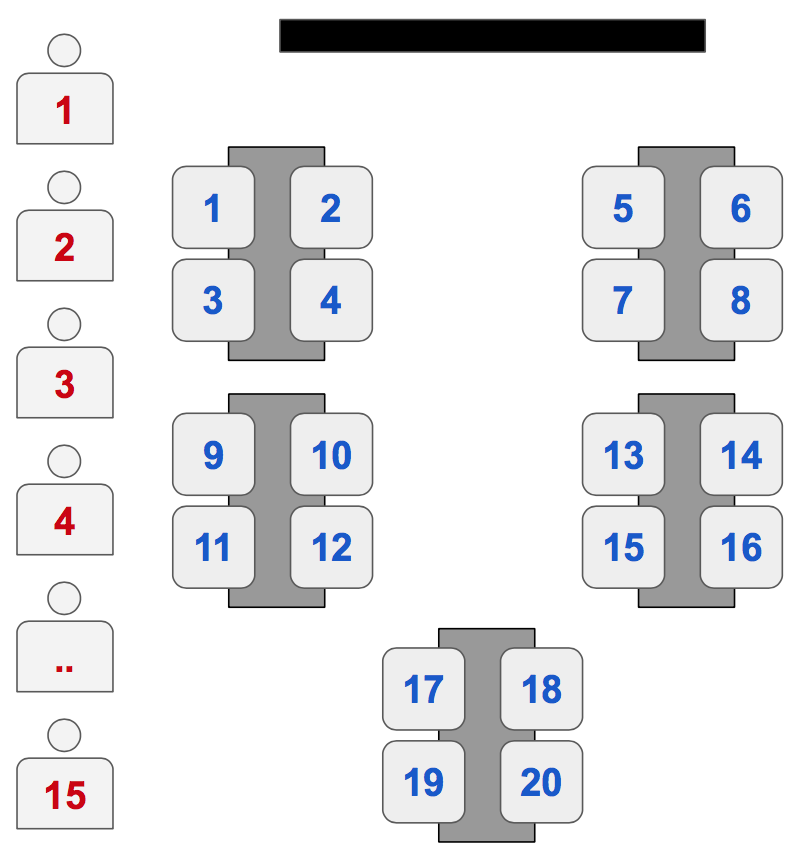
\includegraphics[height=34mm]{images/ssp.png}
}{
  Partly based on slides from Pierre Flener, Barbara Smith and Dimos Tsouros.
}

\begin{frame}{Quick Recap}
  \begin{enumerate}
    \item \inference{Modelling}: express problem in terms of \vfill
      \begin{itemize}
        \item parameters, \vfill
        \item decision variables, with their domains \vfill
        \item constraints, and \vfill
        \item (optionally) objective.
      \end{itemize} \vfill
    \item \search{Solving}: solve using a state-of-the-art solver.
  \end{enumerate}
\end{frame}

\begin{frame}{A Modelling Methodology: Overview}
  \raisebox{-\height}[0pt][0pt]{%
    \begin{columns}
      \begin{column}{0.7\textwidth}

      \end{column}
      \begin{column}{0.3\textwidth}
        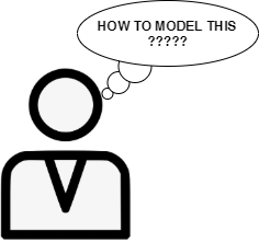
\includegraphics[height=38mm]{images/how_to_model.png}%
      \end{column}
    \end{columns}
  }

  \begin{enumerate}
    \item Make sure you understand the problem correctly:
      \begin{itemize}
        \item What are the knowns (parameters) and unknowns (decision variables)?
        \item What is the objective, if any?
      \end{itemize}
      \vfill
    \item Construct or select some small instance(s) \\of your problem to work with.
      \vfill
    \item Model incrementally:
      \begin{itemize}
        \item Add one constraint at a time and verify that it is correct.
        \item Only add the objective function, if any, at the end.
      \end{itemize}
      \vfill
    \item Model first for correctness and clarity, and only then for efficiency:
      \begin{itemize}
        \item Try to use the most specific type of global constraints which fits
        \item Once you have a correct model, consider \textit{redundant constraints} and symmetries.
          % \item Only as a last resort, add annotations.
      \end{itemize}
      %\item Experiment with different models and different solvers.
  \end{enumerate}
\end{frame}

\begin{frame}{In this lecture}

  We will become an \emph{advanced} modeller!

  Importantly, the same problem can be represented by fundamentally different models.

  \begin{itemize}
    \item The \defined{viewpoint} determines which unknowns to model as decision variables
    \item \defined{Auxiliary} variables are useful, and sometimes required to model complex constraints
    \item \defined{Redundant constraints} can improve the performance of the solver by adding knowledge to the solver which it cannot derive on its own
    \item \defined{Channelling} constraints allow us to combine different viewpoints in the same model
    \item We have a look at some more general modelling guidelines
  \end{itemize}


\end{frame}
\section{Viewpoints}

\newcommand{\taskAllocationDescription}{
  There are three workers (W1, W2, W3).
  Our current project has 4 tasks that have to be allocated to the workers: Construct Product (CP) and Quality Check (QC), which will be conducted on Thursday, and Package Product (PP) and Transport Product (TP), which will be
  conducted on Friday.
  No worker should handle two tasks on the same day.
  Worker W3 cannot work this on Thursday.
  Worker W1 can only perform tasks QC and TP.
}


\ignore{

  \begin{frame}{What is a good model for a constraint problem?}
    You get the problem definition of a constraint problem.
    \parBreak
    \begin{itemize}
      \item You now have to model it \blue{correctly} (and
        \inference{efficiently})!
    \end{itemize}
    \vfill

    How do you choose which of the entities of the problem are the decision variables?
    \vfill

    \begin{example}[Task allocation]
      \taskAllocationDescription
    \end{example}
  \end{frame}

  \begin{frame}{Viewpoints}
    Different models of a problem may result from viewing the problem from different angles or perspectives, \ie different \defined{viewpoints}.
    \vfill

    The \defined{viewpoint} defines the variables and domains of your model.
    \vfill

    \begin{definition}[Law and Lee, 2002]
      A \defined{viewpoint} is a pair \(\langle X, D \rangle\), where \(X = \{x_1, \ldots, x_n\}\) is a set of variables, and \(D\) is a set of domains.
      For each \(x_i \in X\), the associated domain \(D_i\) is the set of possible values for \(x_i\).
      It must be possible to ascribe a meaning to the variables and values of the CSP in terms of the problem \(P\), and so to say what an assignment in the viewpoint \(\langle X, D \rangle\) is intended to represent in terms of \(P\).
    \end{definition}
    \vfill

    \alert{Based on the chosen viewpoint, the size of the search space changes}
  \end{frame}

  \begin{frame}{Viewpoints and size of the search space}

    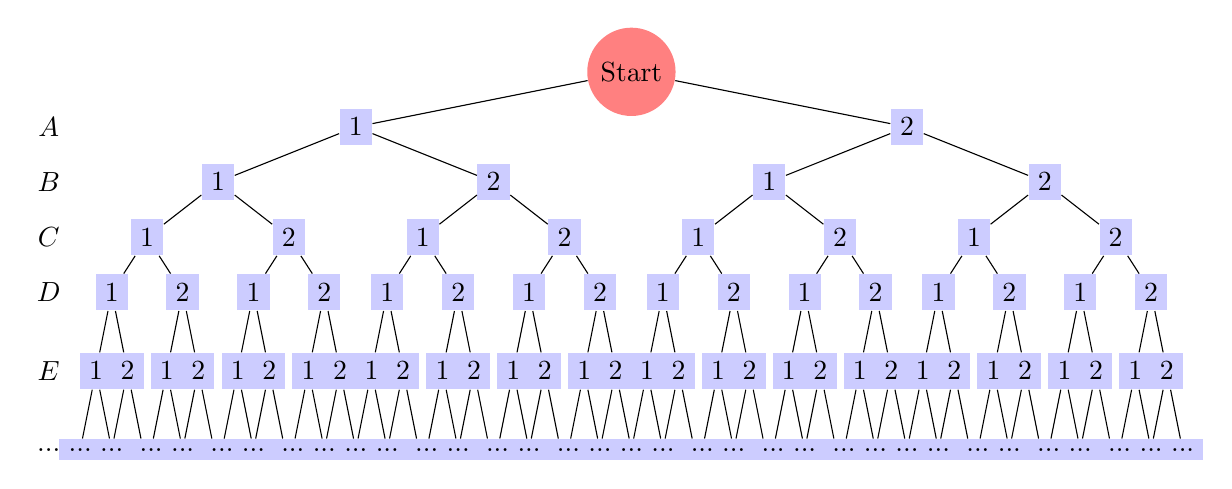
\begin{tikzpicture}[
        val/.style={rectangle, fill=blue!20},
        root/.style={circle, fill=red!50},
        var/.style={rectangle},
        level 1/.style={level distance=0.7cm, sibling distance=7cm},
        level 2/.style={level distance=0.7cm, sibling distance=3.5cm},
        level 3/.style={level distance=0.7cm, sibling distance=1.8cm},
        level 4/.style={level distance=0.7cm, sibling distance=0.9cm},
        level 5/.style={level distance=1cm, sibling distance=0.4cm},
      ]

      % Variables listed on the side
      \coordinate (V) at (-7.4,0);
      \node[var] at (V) { };
      \coordinate (A) at (-7.4,-0.7);
      \node[var] at (A) {$A$};
      \coordinate (B) at (-7.4,-1.4);
      \node[var] at (B) {$B$};
      \coordinate (C) at (-7.4,-2.1);
      \node[var] at (C) {$C$};
      \coordinate (D) at (-7.4,-2.8);
      \node[var] at (D) {$D$};
      \coordinate (E) at (-7.4,-3.8);
      \node[var] at (E) {$E$};
      \coordinate (E) at (-7.4,-4.8);
      \node[var] at (E) {...};

      % Root node and expanded search space with values only
      \node[root] {Start}
      child{node[val]{1} % A=1
        child{node[val]{1} % B=1
          child{node[val]{1} % C=1
            child{node[val]{1} % D=1
              child{node[val]{1}
                child{node[val]{...}}
                child{node[val]{...}}
              } % E=1
              child{node[val]{2}
                child{node[val]{...}}
                child{node[val]{...}}
              } % E=2
            }
            child{node[val]{2} % D=2
              child{node[val]{1}
                child{node[val]{...}}
                child{node[val]{...}}
              } % E=1
              child{node[val]{2}
                child{node[val]{...}}
                child{node[val]{...}}
              } % E=2
            }
          }
          child{node[val]{2} % C=2
            child{node[val]{1} % D=1
              child{node[val]{1}
                child{node[val]{...}}
                child{node[val]{...}}
              } % E=1
              child{node[val]{2}
                child{node[val]{...}}
                child{node[val]{...}}
              } % E=2
            }
            child{node[val]{2} % D=2
              child{node[val]{1}
                child{node[val]{...}}
                child{node[val]{...}}
              } % E=1
              child{node[val]{2}
                child{node[val]{...}}
                child{node[val]{...}}
              } % E=2
            }
          }
        }
        child{node[val]{2} % B=2
          child{node[val]{1} % C=1
            child{node[val]{1} % D=1
              child{node[val]{1}
                child{node[val]{...}}
                child{node[val]{...}}
              } % E=1
              child{node[val]{2}
                child{node[val]{...}}
                child{node[val]{...}}
              } % E=2
            }
            child{node[val]{2} % D=2
              child{node[val]{1}
                child{node[val]{...}}
                child{node[val]{...}}
              } % E=1
              child{node[val]{2}
                child{node[val]{...}}
                child{node[val]{...}}
              } % E=2
            }
          }
          child{node[val]{2} % C=2
            child{node[val]{1} % D=1
              child{node[val]{1}
                child{node[val]{...}}
                child{node[val]{...}}
              } % E=1
              child{node[val]{2}
                child{node[val]{...}}
                child{node[val]{...}}
              } % E=2
            }
            child{node[val]{2} % D=2
              child{node[val]{1}
                child{node[val]{...}}
                child{node[val]{...}}
              } % E=1
              child{node[val]{2}
                child{node[val]{...}}
                child{node[val]{...}}
              } % E=2
            }
          }
        }
      }
      child{node[val]{2} % A=2
        child{node[val]{1} % B=1
          child{node[val]{1} % C=1
            child{node[val]{1} % D=1
              child{node[val]{1}
                child{node[val]{...}}
                child{node[val]{...}}
              } % E=1
              child{node[val]{2}
                child{node[val]{...}}
                child{node[val]{...}}
              } % E=2
            }
            child{node[val]{2} % D=2
              child{node[val]{1}
                child{node[val]{...}}
                child{node[val]{...}}
              } % E=1
              child{node[val]{2}
                child{node[val]{...}}
                child{node[val]{...}}
              } % E=2
            }
          }
          child{node[val]{2} % C=2
            child{node[val]{1} % D=1
              child{node[val]{1}
                child{node[val]{...}}
                child{node[val]{...}}
              } % E=1
              child{node[val]{2}
                child{node[val]{...}}
                child{node[val]{...}}
              } % E=2
            }
            child{node[val]{2} % D=2
              child{node[val]{1}
                child{node[val]{...}}
                child{node[val]{...}}
              } % E=1
              child{node[val]{2}
                child{node[val]{...}}
                child{node[val]{...}}
              } % E=2
            }
          }
        }
        child{node[val]{2} % B=2
          child{node[val]{1} % C=1
            child{node[val]{1} % D=1
              child{node[val]{1}
                child{node[val]{...}}
                child{node[val]{...}}
              } % E=1
              child{node[val]{2}
                child{node[val]{...}}
                child{node[val]{...}}
              } % E=2
            }
            child{node[val]{2} % D=2
              child{node[val]{1}
                child{node[val]{...}}
                child{node[val]{...}}
              } % E=1
              child{node[val]{2}
                child{node[val]{...}}
                child{node[val]{...}}
              } % E=2
            }
          }
          child{node[val]{2} % C=2
            child{node[val]{1} % D=1
              child{node[val]{1}
                child{node[val]{...}}
                child{node[val]{...}}
              } % E=1
              child{node[val]{2}
                child{node[val]{...}}
                child{node[val]{...}}
              } % E=2
            }
            child{node[val]{2} % D=2
              child{node[val]{1}
                child{node[val]{...}}
                child{node[val]{...}}
              } % E=1
              child{node[val]{2}
                child{node[val]{...}}
                child{node[val]{...}}
              } % E=2
            }
          }
        }
      };

    \end{tikzpicture}

    Search space has breadth $d$ and depth $n$, with $d$ being the size of the domains, and $n$ the amount of decision variables used: \textbf{$d^n$ leaves = complete assignments}

  \end{frame}


  \begin{frame}{What is a good model for a constraint problem?}
    \begin{example}[Task allocation]
      \begin{center}
        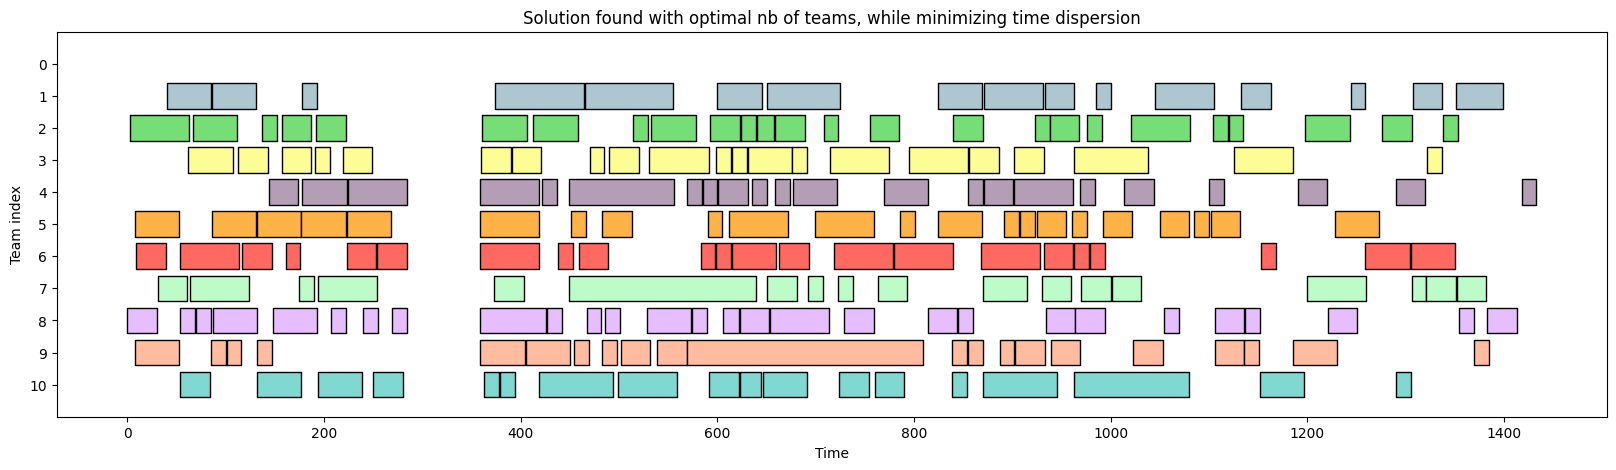
\includegraphics[height=30mm]{images/task_allocation.png}
      \end{center}

      \taskAllocationDescription
    \end{example}
  \end{frame}

  \begin{frame}{What is a good model for a constraint problem?}
    \begin{example}[Task allocation]
      \taskAllocationDescription
    \end{example}

    We have two types of objects: workers $\set{W1, W2, W3}$ and tasks $\set{CP, QC, PP, TP}$.
    For which object should we introduce variables?

    \begin{description}
      \item[Viewpoint 1: Worker variables] For each worker $w_i$, which task(s) are assigned to them?
      \item[Viewpoint 2: Task variables] For each task $t_i$, which worker is assigned to it?
    \end{description}

  \end{frame}

  \begin{frame}{Workers as variables}
    \textbf{Decision Variables}
    One for each worker, so we have 3 variables: $w_1$, $w_2$, and $w_3$
    \parBreak

    \textbf{Initial Domains} A worker can be assigned multiple tasks (over different days).
    So, the domains will be all tasks, but also all pairs of them:
    $
    w_i \in \set{
      \set{},
      \set{CP},
      \set{QC},
      \set{PP},
      \set{TP},
      \set{CP, QC},
      \set{CP, PP},
      \set{CP, TP},\allowbreak
      \set{QC, PP},
      \set{QC, TP},
      \set{PP, TP}
    }, i \in \interval{1}{3}
    $

    Size of the \search{search space}? Domains of size $11$, and $3$ variables: $11^3 = 1331$ assignments.

    \parBreak

    \textbf{Constraints} All tasks have to be assigned to only one
    worker.
    Can we represent it with just pairwise, not equal
    constraints?
    \alert{No}. \\
    \alert{Also, too many unary constraints to model each restriction of the workers.}
  \end{frame}

  \begin{frame}{Tasks are variables}
    \textbf{Decision Variables}
    One for each shift, so we have 4 variables: $t_{CP}, t_{QC}, t_{PP}, t_{TP}$
    \vfill

    \textbf{Initial Domains} Each task has to be assigned to a worker.
    So, the initial domain of every decision variable is the set of workers:
    $t_{CP} \in \set{W1, W2, W3}, \ldots$.
    \vfill

    \textcolor{red}{The problem representation is much easier even
      before formulating the constraints!
    The initial domains are much more straightforward.}
    \vfill

    Size of the \search{search space}?
    Domains of size $3$, and $4$ variables: $3^4 = 81$ assignments.
  \end{frame}

  \begin{frame}{Tasks are variables}
    \textbf{Constraints} Each task has to be assigned to a worker.
    No constraints are needed to represent that now.
    Let's model the unary constraints:
    \vfill

    \begin{enumerate}
      \item No worker should be assigned two tasks in the same day:
        \begin{itemize}
          \item $t_{CP} \neq t_{QC}$
          \item $t_{PP} \neq t_{TP}$
          \item Compare: $(CP \in w_i) \neq (QC \in w_i), i \in \interval{1}{3}$
        \end{itemize}
        \vfill

      \item Worker W3 cannot work this Thursday.
        \begin{itemize}
          \item $t_{CP} \neq W3$
          \item $t_{QC} \neq W3$
          \item Compare: $QP \not \in w_3 \land  CP \not \in w_3$
        \end{itemize}
        \vfill

      \item Worker W1 can only perform tasks QC and TP.
        \begin{itemize}
          \item $t_{CP} \neq W1$
          \item $t_{PP} \neq W1$
          \item Compare: $QC \in w_1 \land TP \in w_2$
        \end{itemize}
    \end{enumerate}
  \end{frame}

}

\newcommand{\nStudents}{\mathtt{nStudents}}
\newcommand{\nChairs}{\mathtt{nChairs}}
\newcommand{\nTables}{\mathtt{nTables}}
\newcommand{\tables}{\mathtt{tables}}
\newcommand{\students}{\mathtt{students}}
\newcommand{\chairs}{\mathtt{chairs}}

\begin{frame}[t]
  \label{studSeat}
  \vfill
  \begin{example}[Student Seating Problem (simplified)]
    \begin{minipage}[c]{0.33\linewidth}
      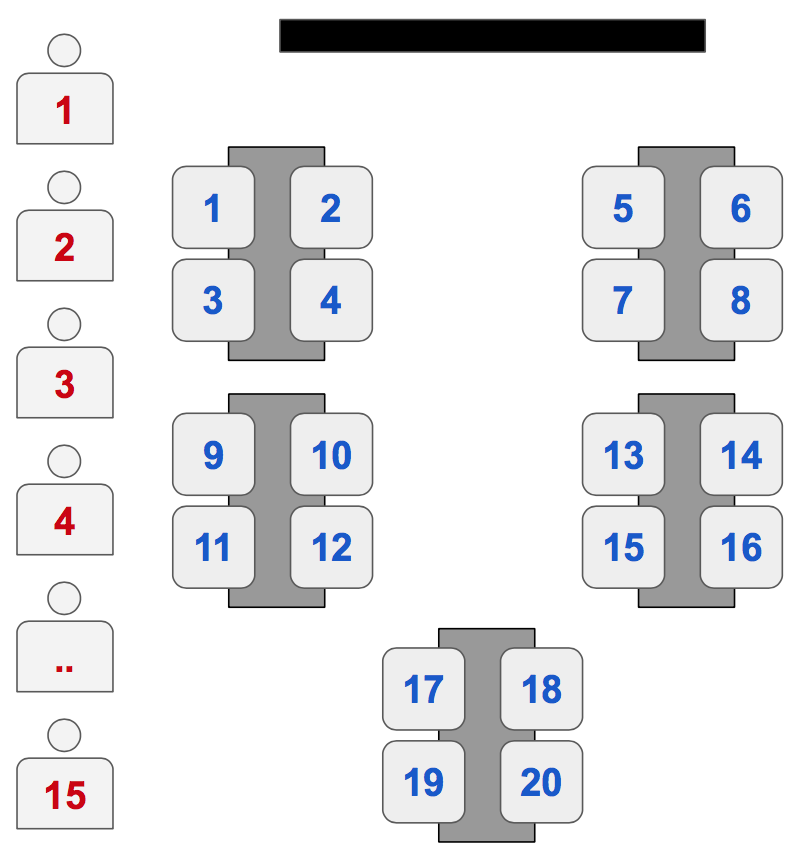
\includegraphics[width=\linewidth]{images/ssp} \\
      \tiny
      $\nStudents = \red{15}$ \\
      $\nChairs = \blue{20} \geq \nStudents$ \\
      $\nTables = 5$ \\
      $\tables = [0..3, 4..7, 8..11, 12..15, 16..19]$
    \end{minipage}
    \hfill
    \begin{minipage}[c]{0.66\linewidth}
      Given:
      \begin{itemize}
        \item $\nStudents$ students,
        \item $\nChairs$ chairs around $\nTables$ tables of four, and
        \item $\mathtt{\tables[i]}$ as the set of chairs of table $i$.
      \end{itemize}

      \parBreak

      Find a seating arrangement such that each table has either at least two of its chairs occupied, or else zero.

      \parBreak
      What are the \stressed{unknowns} of this problem? And what decision variables should we introduce?
    \end{minipage}
  \end{example}
  \vfill
\end{frame}


\begin{frame}{Viewpoints}

  \begin{definition}[Law and Lee, 2002]
    A \defined{viewpoint} is a pair \(\langle X, D \rangle\), where \(X = \{x_1, \ldots, x_n\}\) is a set of variables, and \(D\) is a set of domains.
    For each \(x_i \in X\), the associated domain \(D_i\) is the set of possible values for \(x_i\).
    It must be possible to ascribe a meaning to the variables and values of the CSP in terms of the problem \(P\), and so to say what an assignment in the viewpoint \(\langle X, D \rangle\) is intended to represent in terms of \(P\).
  \end{definition}

  \parBreak

  Here, there are (at least) two \defined{viewpoints}:

  \parBreak

  \begin{description}
    \item[Viewpoint 1] Assign student $i$ to chair $j$
    \item[Viewpoint 2] Assign chair $i$ to student $j$
  \end{description}

  \parBreak
  Which viewpoint will make the problem \emph{easier to model}?
  And which viewpoint will make the problem \emph{easier to solve}?
  Let us try both.

  %
  % Ease of formulating constraints and (optionally) the objective function: Important on choosing the viewpoint to use.
  % \parBreak
  %
  % \begin{itemize}
  %   \item Typically leads also to better \textbf{readability!}
  %   \item This may be very important, depending on the user of the model and their background
  % \end{itemize}
  % \parBreak
  %
  % \alert{But is one viewpoint always clearly the right one to use?}
\end{frame}

\begin{frame}[fragile]{Viewpoint 1: assigning 15 students to 20 chairs}
  Let $\mathtt{\students[i] = j}$ denote that student $i$ is assigned to chair $j$

  \pause
  \parBreak

  % \footnotesize
  % \only<-1>{
  %   \begin{align}
  %     \students_i \in \interval{0}{\nChairs - 1}, &
  %     \quad \forall i \in \interval{0}{\nStudents - 1} \\
  %     \cons{AllDifferent}{\students} \\
  %     \left(\sum_{j \in table, i \in students}{students_i = j}\right) \in
  %     \set{0,2,3,4}, & \forall table \in \tables
  %   \end{align}
  % }
  % \begin{flashcardcpmpy}
  %   \only<2->{
  \lstset{aboveskip=0pt,belowskip=0pt}
  \lstinputlisting[language=cpmpy,firstline=11,lastline=12,numbers=none]{models_cpmpy/t5_student_seating.py}
  \pause
  \lstinputlisting[language=cpmpy,firstline=13,lastline=14,numbers=none]{models_cpmpy/t5_student_seating.py}
  \pause
  \lstinputlisting[language=cpmpy,firstline=15,lastline=21,numbers=none]{models_cpmpy/t5_student_seating.py}
  % }
  % \end{flashcardcpmpy}
  \normalsize
  \vfill

  \pause
  The inner sums have $15 \times 4=60$ terms.

\end{frame}
\begin{frame}[fragile]{Viewpoint 2: assigning 20 chairs to 15 students}
  Let $\mathtt{\chairs[i] = j}$ denote that chair $i$ is assigned to student $j$.
  \pause
  Use $\chairs[i]=-1$ as a \defined{dummy value} to represent that the chair is empty.

  \parBreak

  % \footnotesize
  % \only<-1>{
  % \begin{align}
  %   \chairs_i \in \interval{-1}{\mathtt{nStudents}},
  %   \quad \forall i \in \interval{1}{\mathtt{nChairs}} \\
  %   \cons{AllDifferentExceptN}{\chairs, -1}
  % \end{align}
  % }
  % \begin{flashcardcpmpy}
  %   \only<2->{
  \lstset{aboveskip=0pt,belowskip=0pt}
  \lstinputlisting[language=cpmpy,firstline=25,lastline=26,numbers=none]{models_cpmpy/t5_student_seating.py}
  \pause
  \lstinputlisting[language=cpmpy,firstline=27,lastline=27,numbers=none]{models_cpmpy/t5_student_seating.py}
  \pause
  \lstinputlisting[language=cpmpy,firstline=28,lastline=31,numbers=none]{models_cpmpy/t5_student_seating.py}
  \pause
  \lstinputlisting[language=cpmpy,firstline=32,lastline=33,numbers=none]{models_cpmpy/t5_student_seating.py}
  \pause
%     \begin{lstlisting}[language=output]
% chairs[0] = -1
% chairs[1] = -1
% chairs[2] = -1
% chairs[3] = -1
% chairs[4] = -1
% % [..]
%     \end{lstlisting}
  % \end{flashcardcpmpy}
  \normalsize


  \parBreak
  Although additional constraints are needed, the inner sums have just $4$ terms.
\end{frame}

\begin{frame}

  % Choosing the right viewpoint can make problems \emph{easier to model} and \emph{easier to solve}.
  \parBreak

  The choice of viewpoint will impact how easy certain constraints and objectives are to \inference{model} or \search{solve}.

  \parBreak
  Fortunately, \inference{easier to model} usually means \search{easier to solve} (but not always).

  % Different viewpoints offer different advantages and disadvantages.
  % \parBreak

  \parBreak

  Consider the following when choosing your viewpoint:

  \begin{itemize}
    \item Expressiveness: some constraints or objectives are more easily expressed in one viewpoint than another, which impacts the \stressed{readability} of your model
    \item Performance: what is the strength of the constraints you are providing the solver?
      \begin{itemize}
        \item Does your viewpoint allow for \stressed{strong} global constraints (\eg \con{AllDifferent} over \con{AllDifferentExceptN})
        \item What is the size of the search space?
          \begin{itemize}
            \item Viewpoint 1: $\Oh{\nChairs^{\nStudents}}$
            \item Viewpoint 2: $\Oh{(\nStudents + 1)^{\nChairs}}$
            \item ($(15+1)^{20} \gg 20^{15}$)
          \end{itemize}
        \item Does your viewpoint require you to nest complicated logical (\eg disjunctions) or integer constraints (\eg sub-expressions)?
        \item In general, performance impact is \red{hard} to tell without running experiments!
      \end{itemize}
  \end{itemize}
\end{frame}

\section{Auxiliary variables}

\begin{frame}{Auxiliary variables}
  \begin{definition}
    \defined{Auxiliary variables} are variables that are introduced in the model during the modeling process, and are not necessarily related to entities of our problem.
  \end{definition}
  \vfill
  Auxiliary variables may be useful:
  \begin{itemize}
    \item Expressing constraints may be \textit{easier} using
      auxiliary variables.
    \item Resulting model may be more \textit{readable}.
    \item Propagation of constraints may be more \textit{efficient}.
  \end{itemize}

  \vfill

  Auxiliary variables may be necessary:
  \begin{itemize}
    \item You may not be able to express certain constraints directly using the variables of the chosen \textit{viewpoint}
    \item Depending on the used \textit{solving technology/language}, auxiliary variables may need to be introduced to support nested constraints (using reification).
  \end{itemize}
\end{frame}

\begin{frame}
  % {Auxiliary variables in Table Seating}

  \lstinputlisting[language=cpmpy,firstline=11,lastline=21,numbers=none]{models_cpmpy/t5_student_seating.py}

  An example where auxiliary variables are useful to avoid repeated expressions:
  \pause
  \lstinputlisting[language=cpmpy,basicstyle=\scriptsize,numbers=none,firstline=46,lastline=51]{models_cpmpy/t5_student_seating.py}

  The solver can benefit if the same expression is not introduced twice (although Common Subexpression Elimination (CSE) is in place to do this automatically).
\end{frame}

\newcommand{\yesOption}{\checkmark}
\newcommand{\noOption}{}
\begin{frame}
  \begin{example}[Car Sequencing; Dincbas, Simonis and van Hentenryck, 1988]

    \begin{center}
      Find a \stressed{sequence} in which to produce 10 cars according to the following table:

      \begin{tabular}{|c|c|c|c|c|c|c|c|}
        \hline
        \textbf{Classes}     & \textbf{1} & \textbf{2} & \textbf{3} & \textbf{4} & \textbf{5} & \textbf{6} & \textbf{Cap.} \\
        \hline
        \textbf{No. of cars} & 1          & 1          & 2 & 2          & 2          & 2          &                   \\
        \hline
        \textbf{Option 1}    & \yesOption& \yesOption          & \noOption & \noOption          & \yesOption          & \yesOption          & 1/2               \\
        \hline
        \textbf{Option 2}    & \noOption& \noOption          & \yesOption & \yesOption          & \noOption          & \yesOption          & 2/3               \\
        \hline
        \textbf{Option 3}    & \yesOption& \noOption          & \noOption & \noOption          & \yesOption          & \noOption          & 1/3               \\
        \hline
        \textbf{Option 4}    & \yesOption& \yesOption          & \noOption & \yesOption          & \noOption          & \noOption          & 2/5               \\
        \hline
        \textbf{Option 5}    & \noOption& \noOption          & \yesOption & \noOption          & \noOption          & \noOption          & 1/5               \\
        \hline
      \end{tabular}
    \end{center}

    \begin{itemize}
      \item The \stressed{class} of each car determines how many cars to produce, and with which options. \Eg for class 1, we should produce 1 car with options 1, 3, and 4.
        \begin{itemize}
          \item \Eg a sequence of car classes: $\sequence{1,2,3,3,4,4,5,5,6,6}$
        \end{itemize}
      \item The stations that install the options have limited \stressed{capacities}. \Eg for option 1, we can only produce 1 car in every sub-sequence of 2 cars. Producing a car of class 1 can thus only be directly followed by a car of class 3 or 4.
    \end{itemize}

    % \begin{columns}
    %   \begin{column}{0.30\textwidth}
    %     \begin{itemize}
    %         % \item Each car of class requires some options, e.g. car 1 requires options 1, 3, and 4.
    %         %        \item Options are installed at stations, which have lower capacity than rest of line e.g. at most 1 car out of 2 for option 1
    %         %        \item Find a feasible production sequence
    %     \end{itemize}
    %   \end{column}
    %   \begin{column}{0.7\textwidth}
    %     \begin{center}
    %     \end{center}
    %   \end{column}
    % \end{columns}
  \end{example}
\end{frame}

\begin{frame}{Auxiliary variables - Car Sequencing}
  % Add the image at the top right corner
  \raisebox{-\height}[0pt][0pt]{%
    \begin{columns}
      \begin{column}{0.7\textwidth}

      \end{column}
      \begin{column}{0.3\textwidth}
        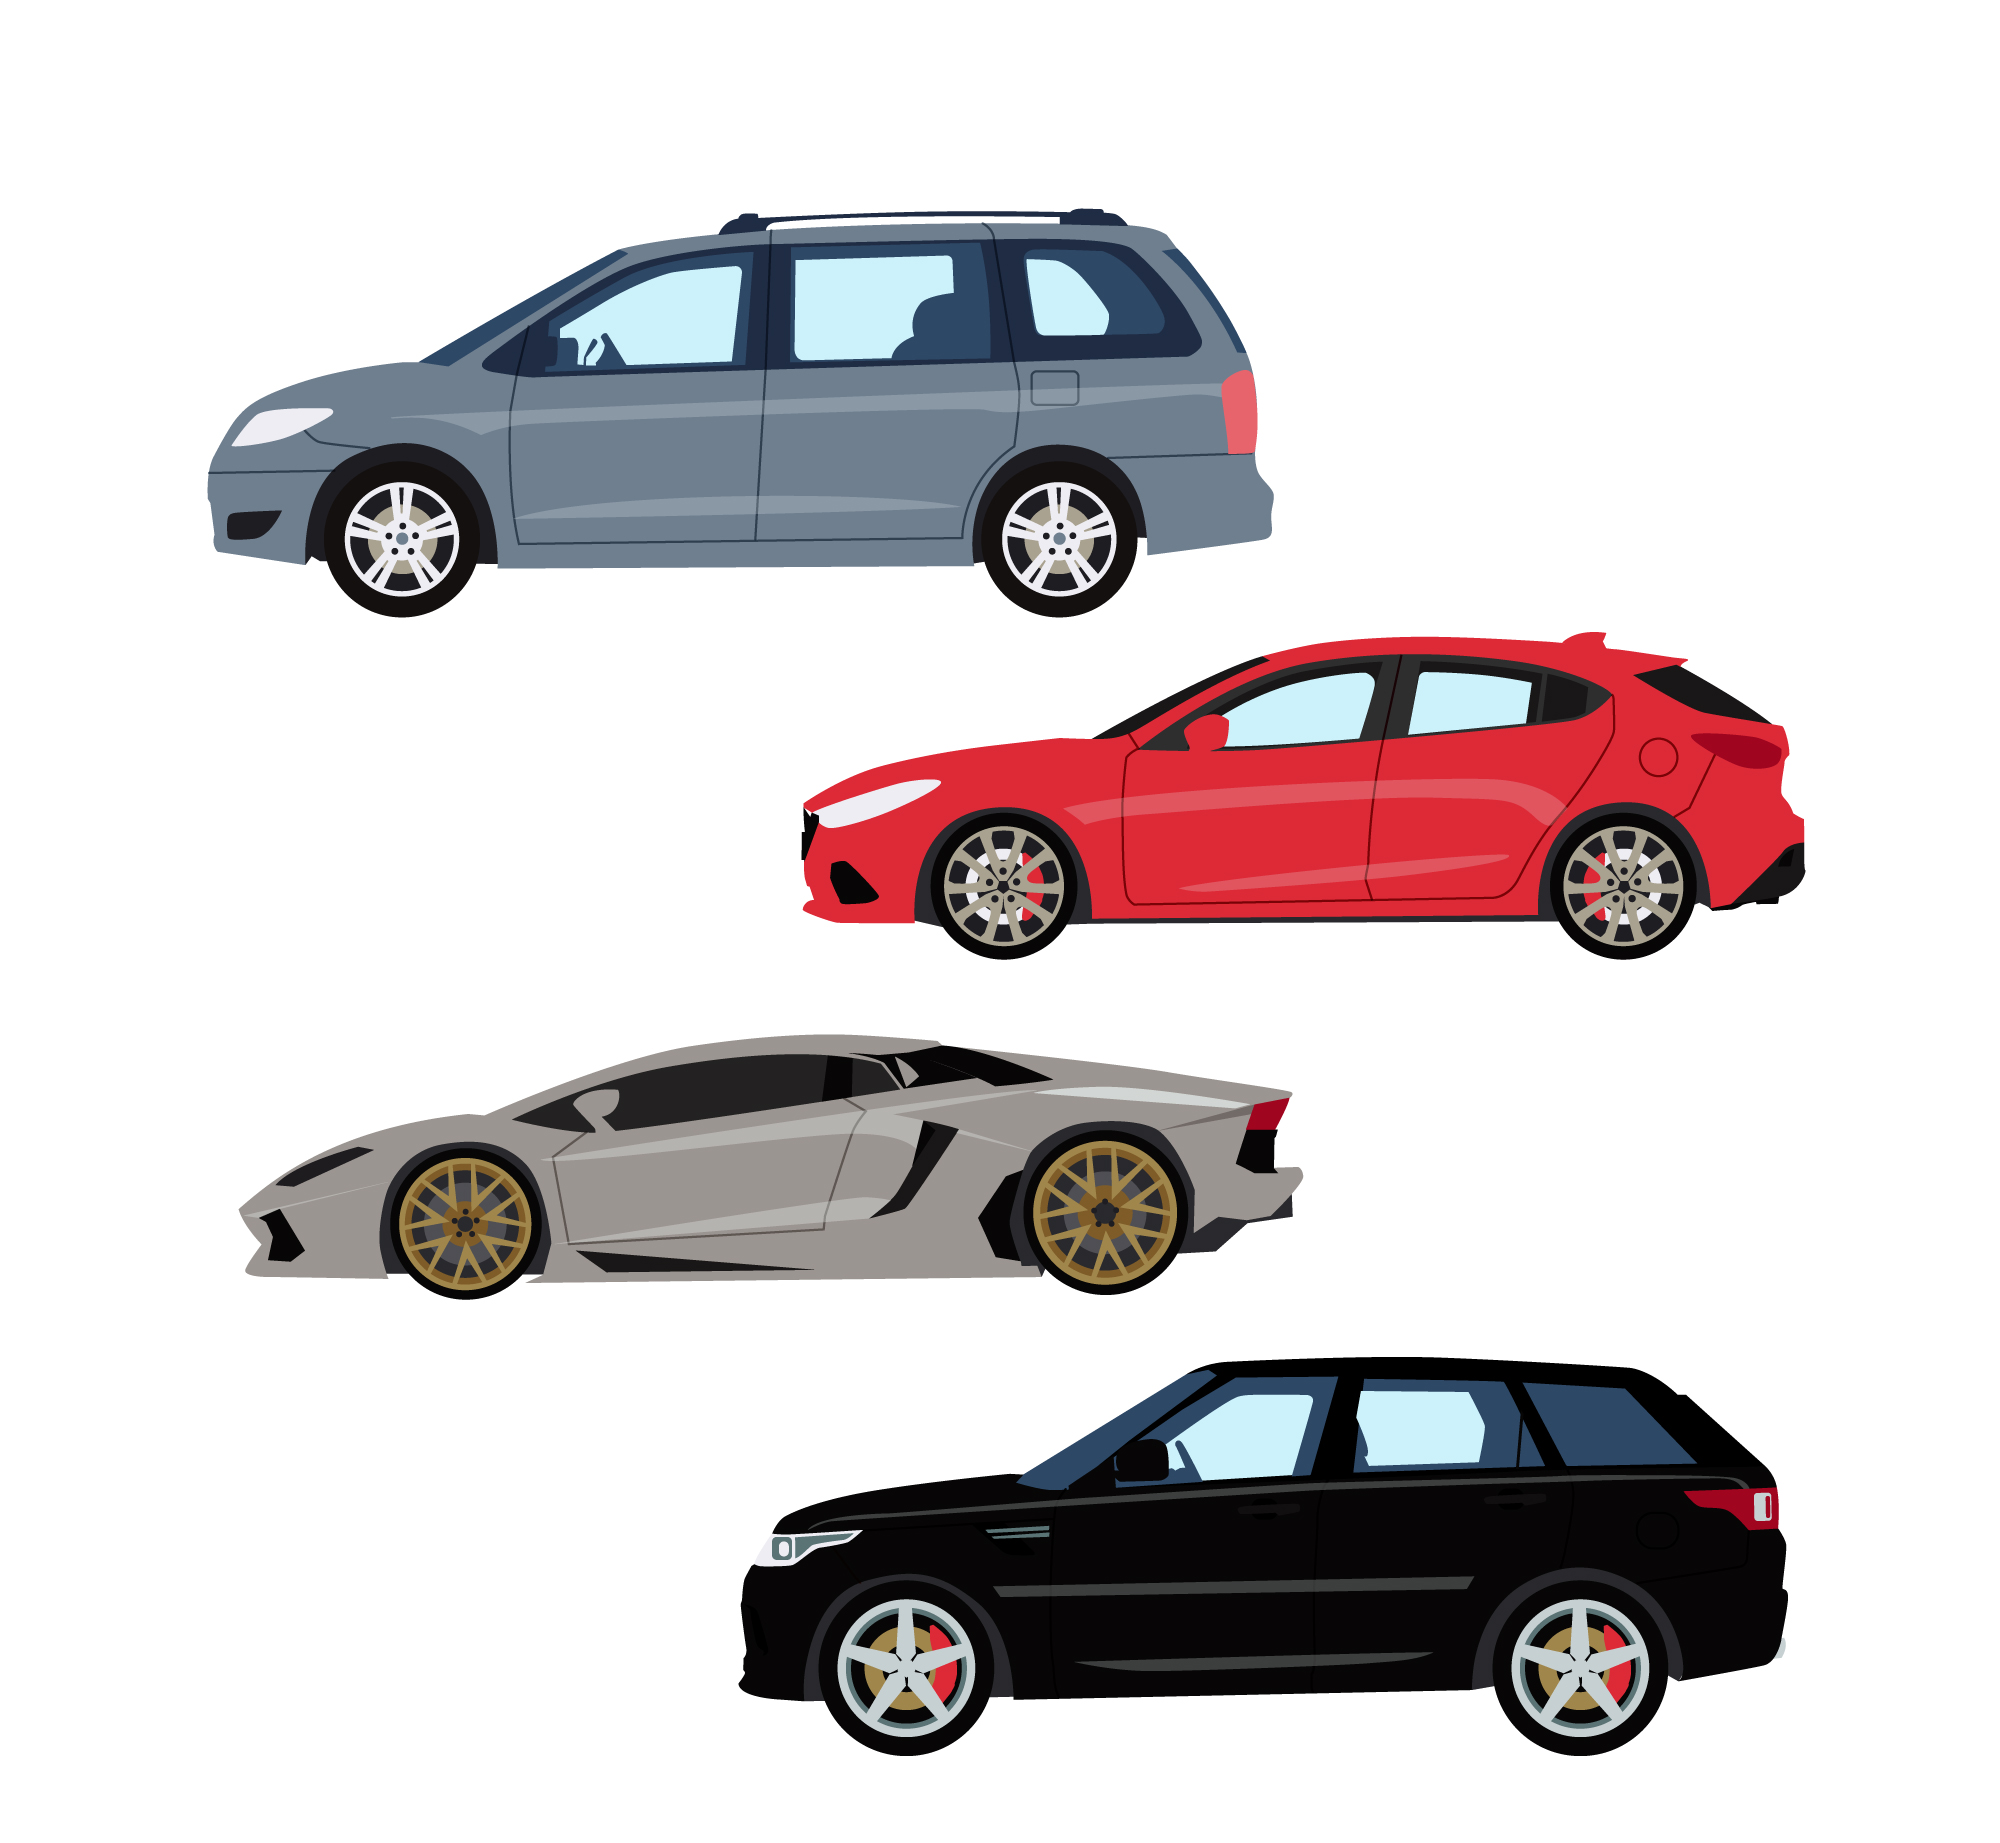
\includegraphics[height=35mm]{images/car_seq.png}%
      \end{column}
    \end{columns}
  }

  \begin{itemize}
    \item Viewpoint:
      \begin{itemize}
        \item A variable for each position in the sequence, \\
          \(s_1, s_2, \ldots, s_{10} \in S\)

        \item Let \(s_i = j\) denote that the $i$-th car is of class $j$
      \end{itemize}
      \vfill

    \item Constraints:
      \begin{itemize}
        \item Each class occurs the correct number of times
          $\cons{Count}{s, k} = d_k \quad \forall k \in \mathtt{Classes}$ \\
          with $d_k$ being the production demand for class $k$.
          This posts \eg $\cons{Count}{s, 3} = 2$ to ensure we build 2 cars of class 3.

          \parBreak

          \inference{Or better}: $GlobalCardinalityCount(S, Classes, D)$

          with $D$ being the list of production demands for each class.
          \parBreak

        \item How to model the option given the capacities? This is (almost) impossible given the current viewpoint.
      \end{itemize}
  \end{itemize}

  % \vfill
  % \alert{Cannot model the option capacities directly by using
  %   variables $s_i$!  (Actually we can, with a long and complex
  % constraint that will create auxiliary variables either way)}
  % \vfill
\end{frame}

\begin{frame}{Auxiliary variables - Car Sequencing}

  % Add the image at the top right corner
  \raisebox{-\height}[0pt][0pt]{%
    \begin{columns}
      \begin{column}{0.7\textwidth}

      \end{column}
      \begin{column}{0.3\textwidth}
        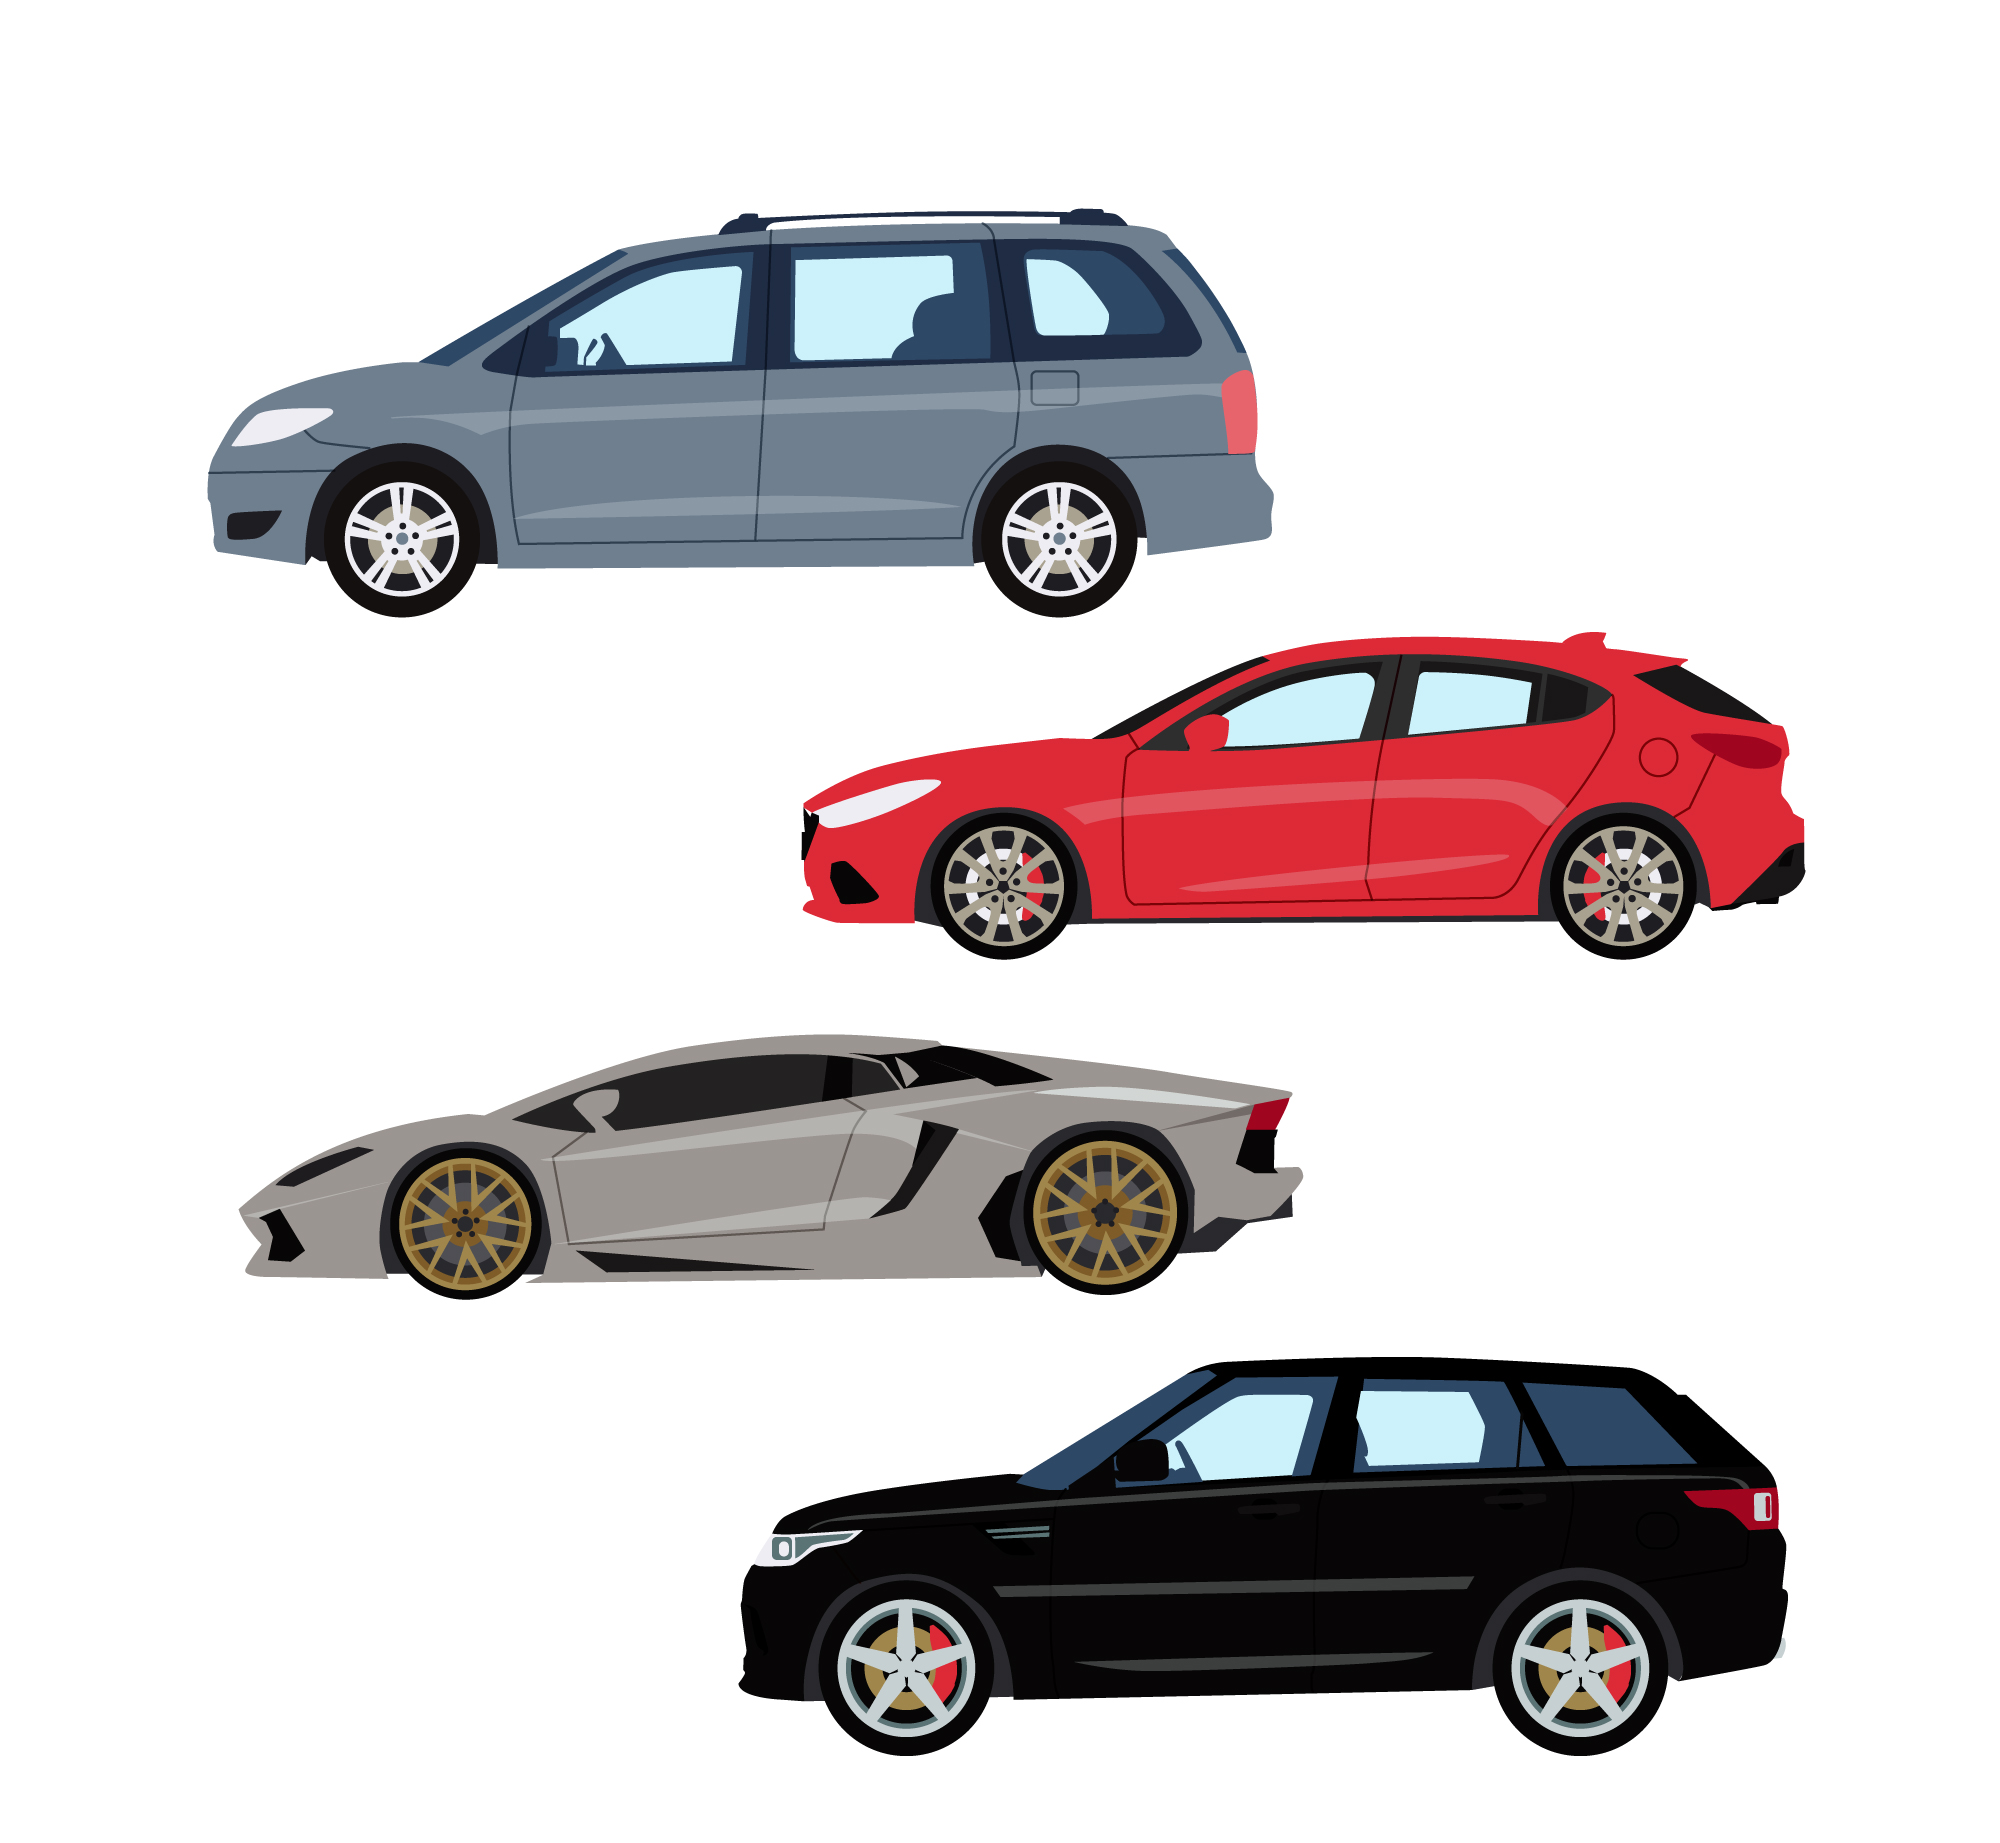
\includegraphics[height=35mm]{images/car_seq.png}%
      \end{column}
    \end{columns}
  }

  How can we model the constraints for the option capacities?
  \vfill

  \begin{itemize}
    \item Introduce \defined{auxiliary} variables \(o_{ij}\):
      \begin{itemize}
        \item \(o_{ij} = 1\) iff the car in the \(i\)-th slot in the sequence requires option \(j\)
      \end{itemize}
      \vfill

      \pause
    \item Capacity constraint for \eg option 2 with capacity of 2/3
      \begin{itemize}
        \item Constrain a sliding window of size 3
        \item \(o_{i,2} + o_{i+1,2} + o_{i+2,2} \leq 2 \quad \text{for} \quad 1
          \leq i \leq 8\)
      \end{itemize}
      \vfill
      \pause

    \item Relate the auxiliary variables to the \(s_i\) variables:
      \begin{itemize}
        \item Matrix \(\lambda_{kj} = 1\) if car class \(k\) requires option \(j\)
        \item If $s_i = k$, then the options of class $k$ are required in slot $i$
        \item \(o_{ij} = \lambda_{s_i j} \quad 1 \leq i \leq 10, \, 1 \leq j \leq 5\)
          \alert{Note: this uses in practice the
            \texttt{Element} global function. A variable ($s_i$) is used as
          index into the rows of $\lambda$.}
      \end{itemize}
  \end{itemize}
\end{frame}

\begin{flashcardcpmpy}
  \begin{frame}{Auxiliary variables -- Car Sequencing -- CPMpy}
    \begin{example}[CPMpy model for Car Sequencing (indexing offset 0)]
      \lstinputlisting[language=cpmpy,basicstyle=\scriptsize,numbers=none,firstline=13,lastline=29]{models_cpmpy/car_sequencing.py}
    \end{example}
  \end{frame}
\end{flashcardcpmpy}

\section{Redundant Constraints}

\begin{frame}{Redundant constraints}
  We have chosen a viewpoint, and formulated the constraints to express our problem in a \blue{correct} and \stressed{readable} model. But, can we do something to make the solving more \inference{efficient}?
  \parBreak

  During the search process, the solver will explore several infeasible parts of the search tree when it cannot propagate constraints. Can we avoid that?
  \parBreak

  \redundantConstraintDefinition
  \parBreak

  Although \defined{redundant} constraints are logically redundant,
  and do not change the set of solutions, they can be used to
  \blue{reduce the search effort of the solving process}.
\end{frame}

\begin{frame}{Redundant constraints}
  \begin{example}
    Because of the viewpoint, it is impossible to assign more than four students to the same table. However, we can add the following redundant constraint:

    \lstinputlisting[language=cpmpy,basicstyle=\scriptsize,numbers=none,firstline=51,lastline=51]{models_cpmpy/t5_student_seating.py}
  \end{example}

  % \begin{definition}
  %   \defined{Redundant constraints}, also called \textit{implied}
  %   constraints, are constraints which are entailed by the
  %   constraints defining the problem. They do not change the set of
  %   solutions, and hence are logically redundant.
  % \end{definition}
  % \vfill

  Redundant constraints are often added to the model to reduce the search effort, by \red{cutting infeasible parts} of the search tree early.
  So the solver does not need to explore possible assignments in these subproblems.

  \begin{itemize}
    \item at some point during search, we will have a partial
      assignment that cannot lead to a solution
    \item the redundant constraint can detect inconsistency of the
      partial assignment
      \begin{itemize}
        \item the redundant constraint forbids it, but \textbf{does
          not change the set of solutions}
      \end{itemize}
    \item while without the redundant constraint, the search would
      continue deeper
  \end{itemize}
\end{frame}

\begin{frame}{Redundant constraints -- Car Sequencing}
  % Add the image at the top right corner
  \raisebox{-\height}[0pt][0pt]{%
    \begin{columns}
      \begin{column}{0.7\textwidth}

      \end{column}
      \begin{column}{0.3\textwidth}
        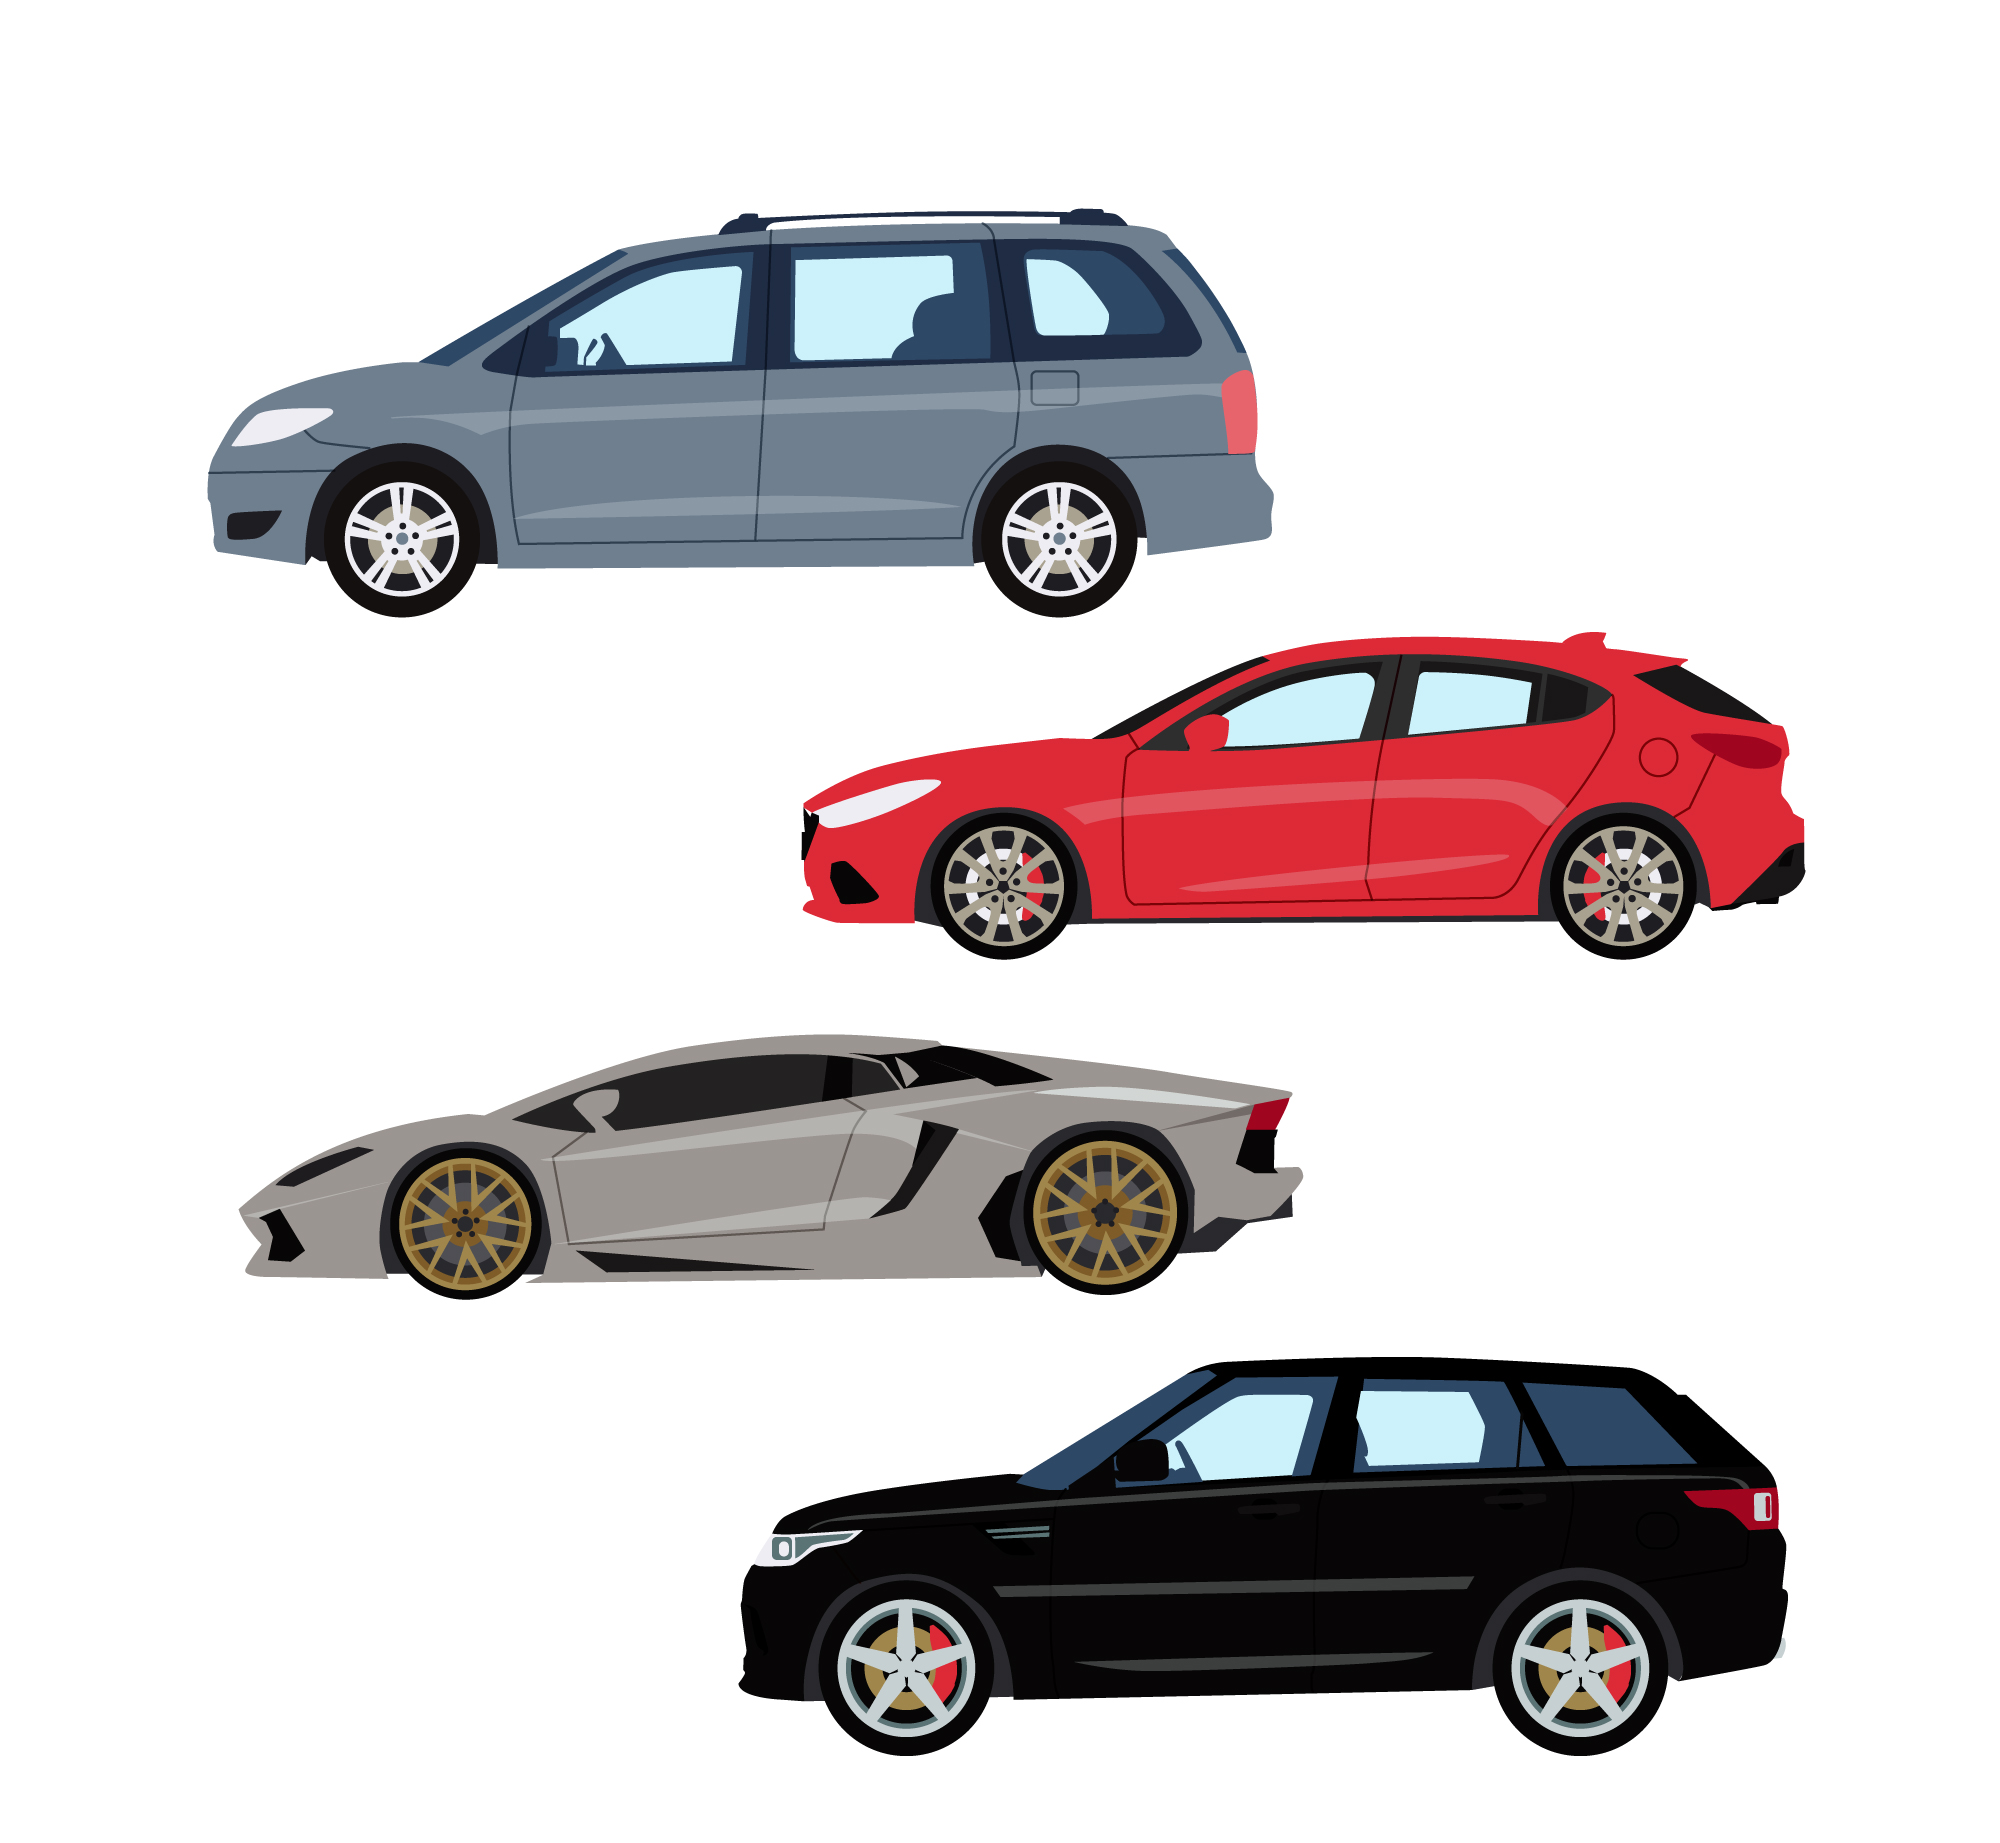
\includegraphics[height=35mm]{images/car_seq.png}%
      \end{column}
    \end{columns}
  }

  \begin{itemize}
    \item Existing constraints only say that the option capacities
      \\ cannot be \emph{exceeded}
      \begin{itemize}
        \item but we can’t stay too far below capacity either
      \end{itemize}
      \vfill

    \item Suppose there are 30 cars, and 12 require option 1
      \vfill

    \item Reminder: Option 1 capacity is 1 car in 2
      \vfill

    \item At least one car in slots 1 to 8 of the production sequence
      \\ must have option 1
      \begin{itemize}
        \item otherwise 12 of cars 9 to 30 will require option 1,
          i.e. too many
      \end{itemize}
      \vfill

    \item Cars 1 to 10 must include at least two option 1 cars,
      \ldots, and cars 1 to 28 must include at least 11 option 1 cars
      \vfill

    \item These are \emph{redundant constraints} that can be used to
      speed up search in car sequencing
  \end{itemize}
\end{frame}

\begin{frame}
  \begin{example}[Magic Series of length \texttt{n}]
    The element at index \texttt{i} in \texttt{I = 0..(n-1)} is
    the number of occurrences of \texttt{i}.
    A solution for $\mathtt{n}=4$: $\mathtt{Magic}=[1,2,1,0]$ (0 occurs once, 1 occurs twice, ...)
    \parBreak

    \structured{Decision variables:} \quad \texttt{Magic} ~=~
    \begin{tabular}{cccc}
      \texttt{0}                             & \texttt{1} & $\cdots$
      & \texttt{n-1} \\
      \hline
      \multicolumn{1}{|c|}{$\in \mathtt{I}$} &
      \multicolumn{1}{|c|}{$\in \mathtt{I}$} &
      \multicolumn{1}{|c|}{$\cdots$}         &
      \multicolumn{1}{|c|}{$\in \mathtt{I}$}
      \\
      \hline
    \end{tabular} \\~\\

    \small
    \structured{Problem Constraint:}
    \only<-1>{
      \[ \forall i \in I, \quad \text{Magic}[i] = \sum_{j \in I}
      (\text{Magic}[j] = i) \]
      or, logically equivalently but better:
      \[ \forall i \in I, \quad \text{CountEq}(\text{Magic}, i,
      \text{Magic}[i]) \]
      or, logically equivalently and even better:
      \[ \text{GlobalCardinalityCount}(\text{Magic}, \text{array1d}(I,
      [i \mid i \in I]), \text{Magic}) \]
    }

    \begin{flashcardcpmpy}
      \only<2->{
        \begin{center}
          \cpminline{[Magic[i] == cp.sum(Magic == i) for i in range(len(Magic))]}
        \end{center}
        or, logically equivalently but better:
        \begin{center}
          \cpminline{[Magic[i] == cp.Count(Magic, i) for i in range(len(Magic))]}
        \end{center}
        or, logically equivalently and even better:
        \begin{center}
          \cpminline{cp.GlobalCardinalityCount(Magic, range(len(Magic)), Magic)}
        \end{center}
      }
    \end{flashcardcpmpy}
  \end{example}
\end{frame}

\begin{frame}{Redundant constraints}
  We have modeled the problem correctly.
  Example solutions: $\mathtt{Magic}=[1,2,1,0], [2,0,2,0], \ldots$.
  What redundant constraints can we add?
  \parBreak

  \structured{Redundant Constraints:} \quad $\sum \text{Magic} = \pause n$ and $\sum_{i \in I} (i \times \text{Magic}[i]) = \pause n$

  % \begin{align*}
  %   \sum \text{Magic} = & \only<-1>{?}\only<2->{n & \quad & \text{Sum up counts of occurrences}}   \\
  %   \sum_{i \in I} (i \times \text{Magic}[i]) = & \only<-1>{?}\only<3->{n & \quad & \text{More tricky!}}
  % \end{align*}

  \parBreak
  The first holds because we sum up counts of occurrences of each number, and there are $n$ numbers.

  \parBreak
  % TODO this can be removed "made homework" if too complex to explain
  The second is more tricky. Because $\text{Magic}[i] = j$ means there are $j$ occurrences of value $i$, placed at some indices $k_1, \ldots, k_j$, which in turn ensures $\text{Magic}[k_1], \ldots, \text{Magic}[k_j]$ numbers are placed.
  However, now we are counting occurrences again ($\text{Magic}[k_1]$ number of $k_1$'s, etc.), which always should add up to $n$.

  \parBreak
  Depending on the formulation above of the problem constraint, the redundant constraints can accelerate a CP solver up to $100$ times for $\mathtt{n}=150$.
\end{frame}

\begin{frame}{Redundant Constraints}
% Add the image at the top right corner
\raisebox{-\height}[0pt][0pt]{%
  \begin{columns}
    \begin{column}{0.7\textwidth}

    \end{column}
    \begin{column}{0.3\textwidth}
      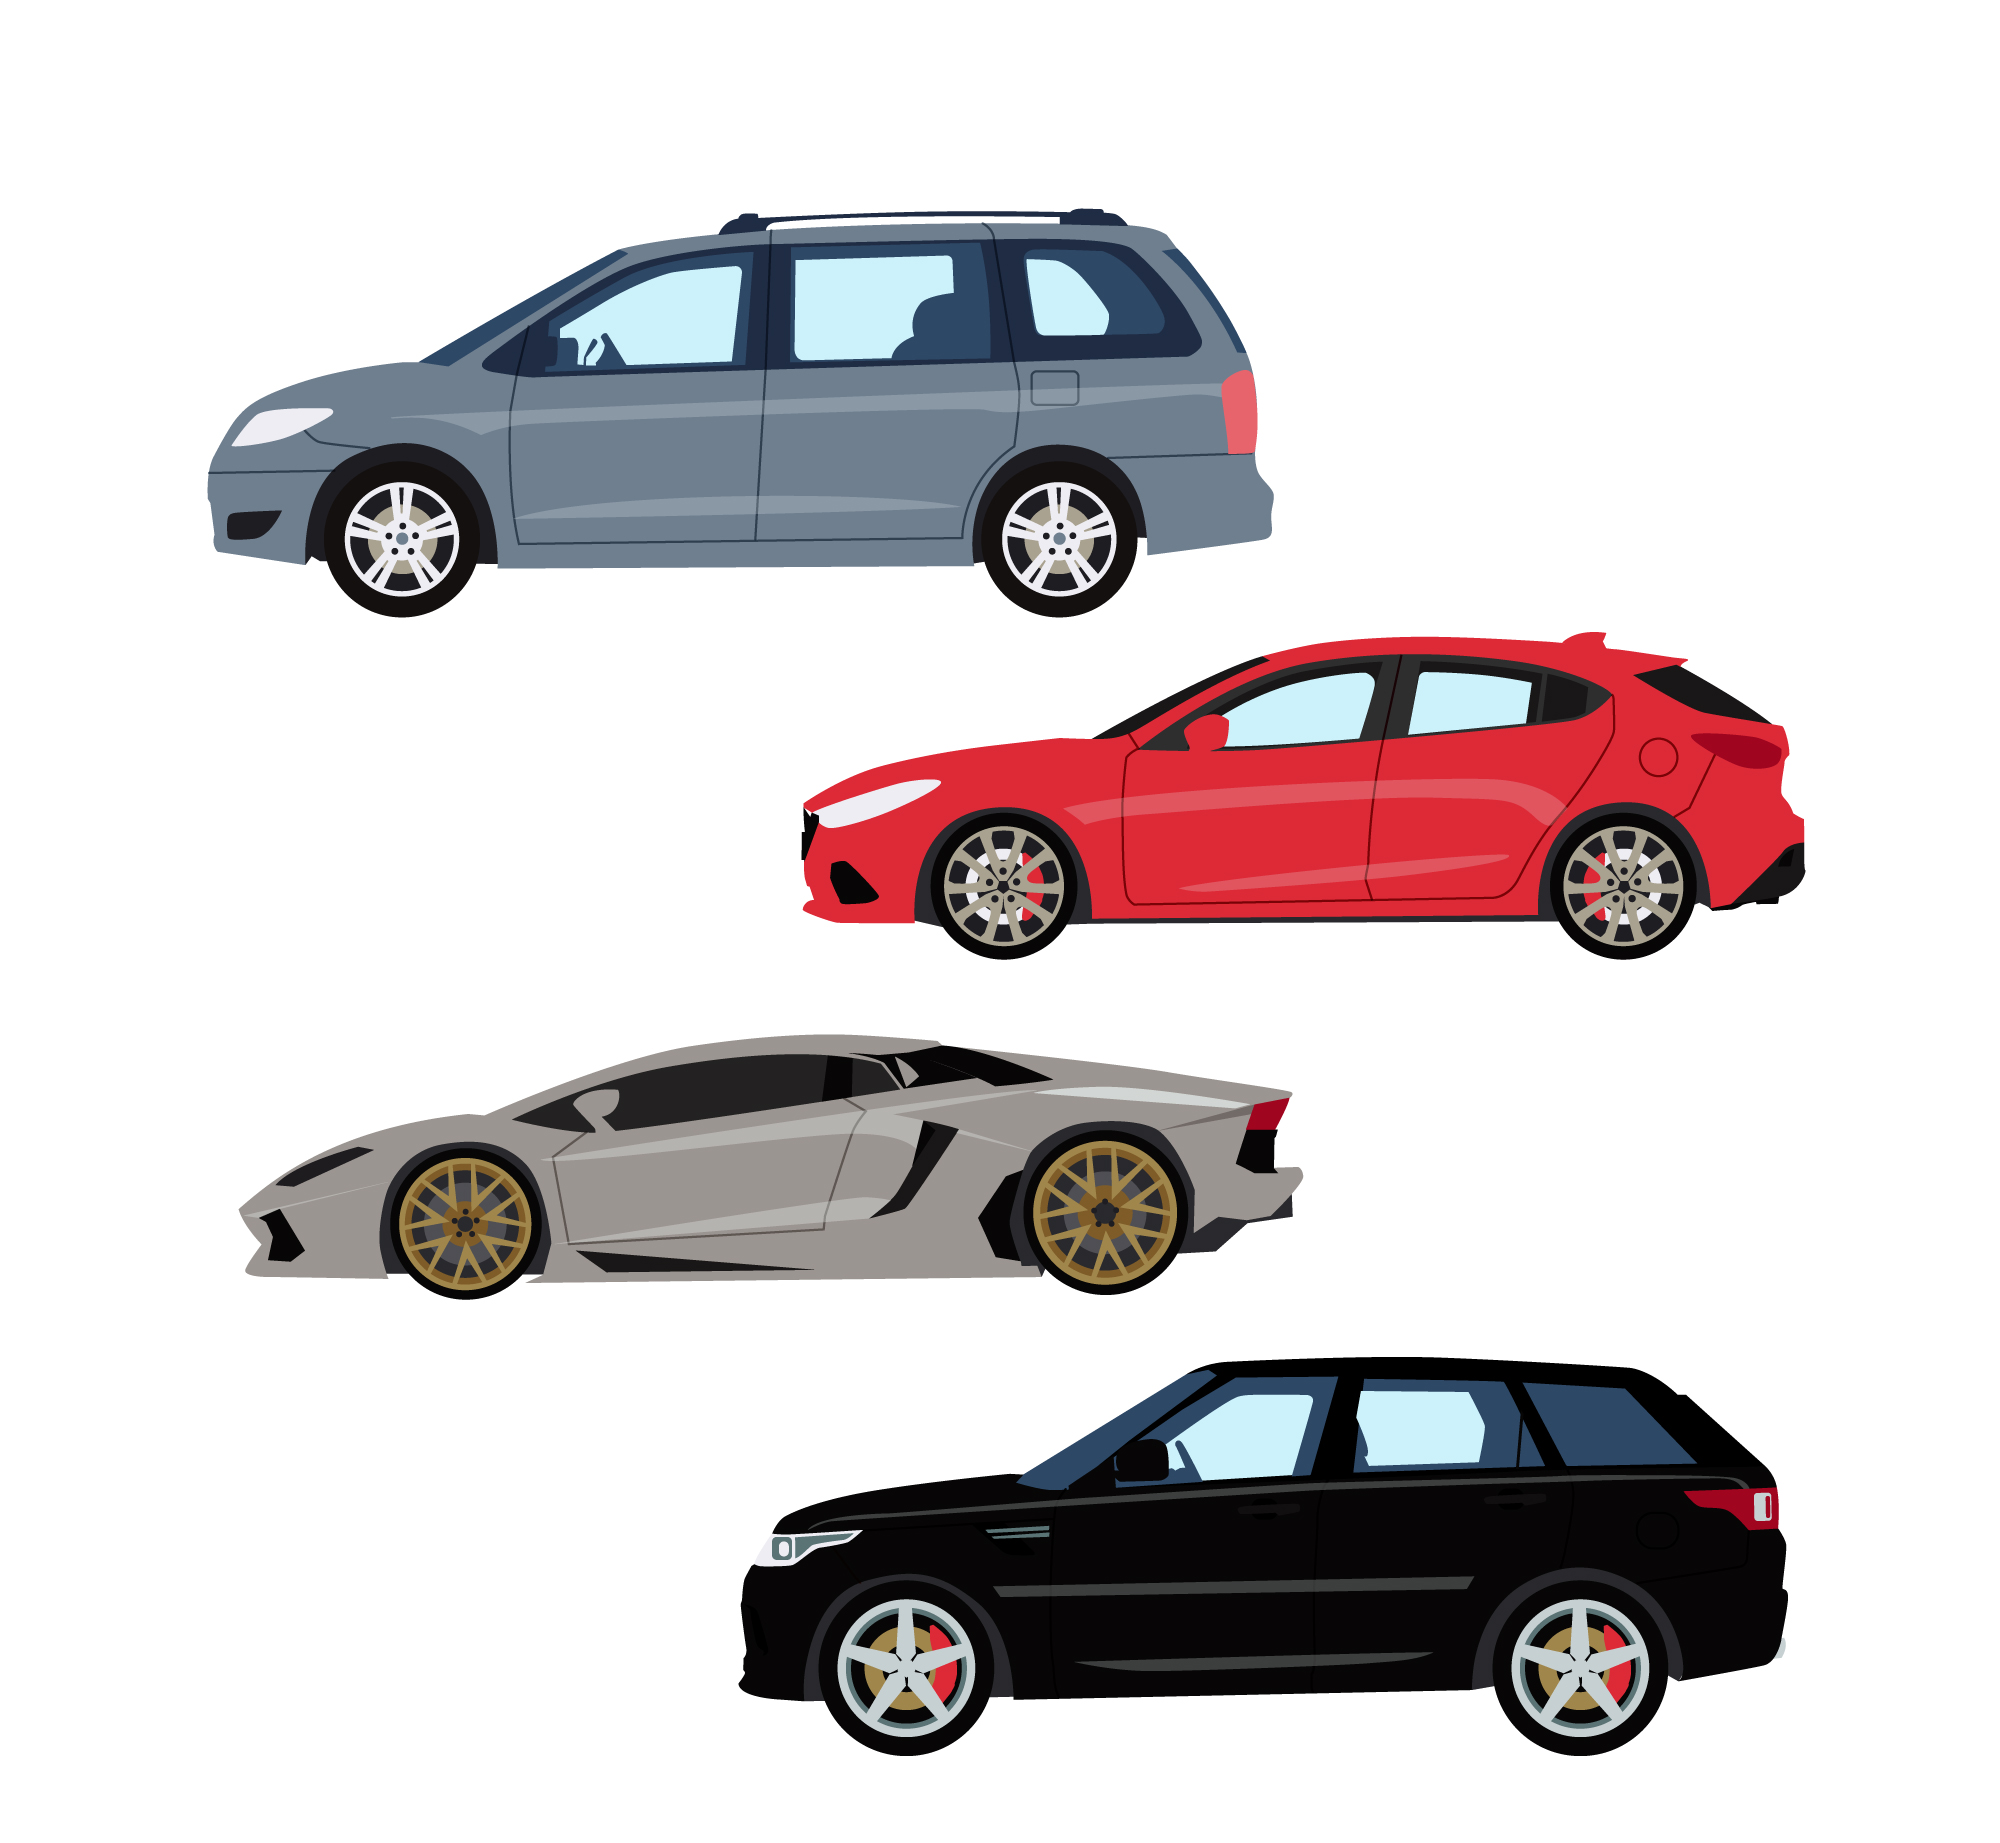
\includegraphics[height=35mm]{images/car_seq.png}%
    \end{column}
  \end{columns}
}

\alert{Be careful though: not all redundant constraints
\\accelerate the solving.}
\vfill

\begin{itemize}
  \item The assignments forbidden by a redundant constraint \\ may
    never actually arise during search
    \begin{itemize}
      \item This means more propagation time and no benefit
    \end{itemize}
    \vfill

  \item \Eg in car sequencing,
    \begin{itemize}
      \item at least one of the first 8 cars must require option 1 ($o_{1,1} + o_{2,1} + o_{3,1} + \ldots + o_{8,1} \geq 1$)
      \item in general, \emph{any} 8 consecutive cars must have one option 1 car
      \item but this redundant constraint is quite weak, and is thus less likely to pay off
    \end{itemize}
    \vfill

  \item If we find a \emph{class} of redundant constraints, maybe only some are useful
    \begin{itemize}
      \item adding a lot of constraints that don’t reduce search will increase the run-time
    \end{itemize}
\end{itemize}
\end{frame}

\section{Combining viewpoints: Redundant Variables \& Channelling}

\begin{frame}{Combining viewpoints}
Adding \defined{auxiliary} variables may be important to model your
problem (efficiently), while adding \defined{redundant constraints}
can speed up the search process.
\vfill

\blue{Can we do something more to get a more efficient model??}
\vfill

We may have spotted different viewpoints for our problem \dots
\vfill

And one is not \textit{clearly}  better than the other: \\
Different perspectives often allow different expression of the
constraints and different redundant constraints
\vfill

\green{Why choose one of them? Can use both!}
\end{frame}

\begin{frame}{Combining viewpoints}
We have chosen our main viewpoint for the problem,\\
\begin{itemize}
  \item but we also introduce a second viewpoint with the hope that
    it will help in propagation during search.
\end{itemize}
\vfill

This means we will use \defined{redundant variables}, that do not
capture information not already captured in the model.
\begin{definition}
  A \defined{redundant decision variable} denotes information
  already denoted by other
  % decision
  variables: \defined{mutual redundancy} (same information) vs
  \defined{non-mutual redundancy}.
\end{definition}\vfill

The constraints of the second viewpoint will be used on these variables.
\end{frame}

\begin{frame}{Channelling}
Including the variables and constraints of both viewpoints may
allow the solver to infer different things from each one, and
reduce the search space.
\vfill

But we have to make sure that our 2 sets of variables solve the
same problem!
\vfill

\alert{We need to channel the 2 viewpoints}, linking the variables
i.e. make sure that assignments (and domain pruning) on one
viewpoint are propagated to the other.
\vfill

\begin{definition}
  A \defined{channelling constraint} fixes the value of 1 set of decision variables when the values of the decision variables they are redundant with from the second set are fixed.
  Channelling can be \defined{1-way} (one viewpoint determines the other) or \defined{2-way} (assignments and domain pruning propagate in both directions).
\end{definition}
\end{frame}

\begin{frame}{Channelling }
\begin{example}[Golomb Rulers]
  \begin{columns}
    \begin{column}{0.6\textwidth}

      \begin{itemize}
        \item A Golomb ruler with \(m\) marks consists of:
          \begin{itemize}
            \item a set of \(m\) integers \(x_1, x_2, \ldots, x_m\) (marks on the ruler)
            \item all differences $x_j - x_i$ (for $i < j$) are all different
            \item Objective: find ruler with minimum length \(\max_i x_i\)
          \end{itemize}
          \vfill

        \item First viewpoint: ordered marks \(0 = x_1 < x_2 < \ldots < x_m\)
          \begin{itemize}
            \item $\cons{AllDifferent}{\set{x_j - x_i : 1 \leq i < j \leq m}}$
            \item \(x_1 < x_2 < \ldots < x_m\) \\
              {\small (marks are unordered in the problem; ordering is a modelling choice --- also symmetry breaking, next lecture)}
          \end{itemize}
          \vfill

          % \item Second viewpoint: \textit{difference} variables \(d_{ij}, \, 1 \leq i < j \leq m\)
        \item Second viewpoint: \(d_{ij}, \, 1 \leq i < j \leq m\)
          \begin{itemize}
            \item $\cons{AllDifferent}{{\set{d_{ij} : 1 \leq i < j \leq m}}}$
            \item \(d_{ik} = d_{ij} + d_{jk} \quad \text{for } 1 \leq i
              < j < k \leq m\)
          \end{itemize}
          \vfill
        \item \stressed{Channelling} constraints: \(d_{ij} = x_j - x_i\)
      \end{itemize}
    \end{column}
    \begin{column}{0.3\textwidth}
      \begin{center}
        \vfill
        \begin{figure}
          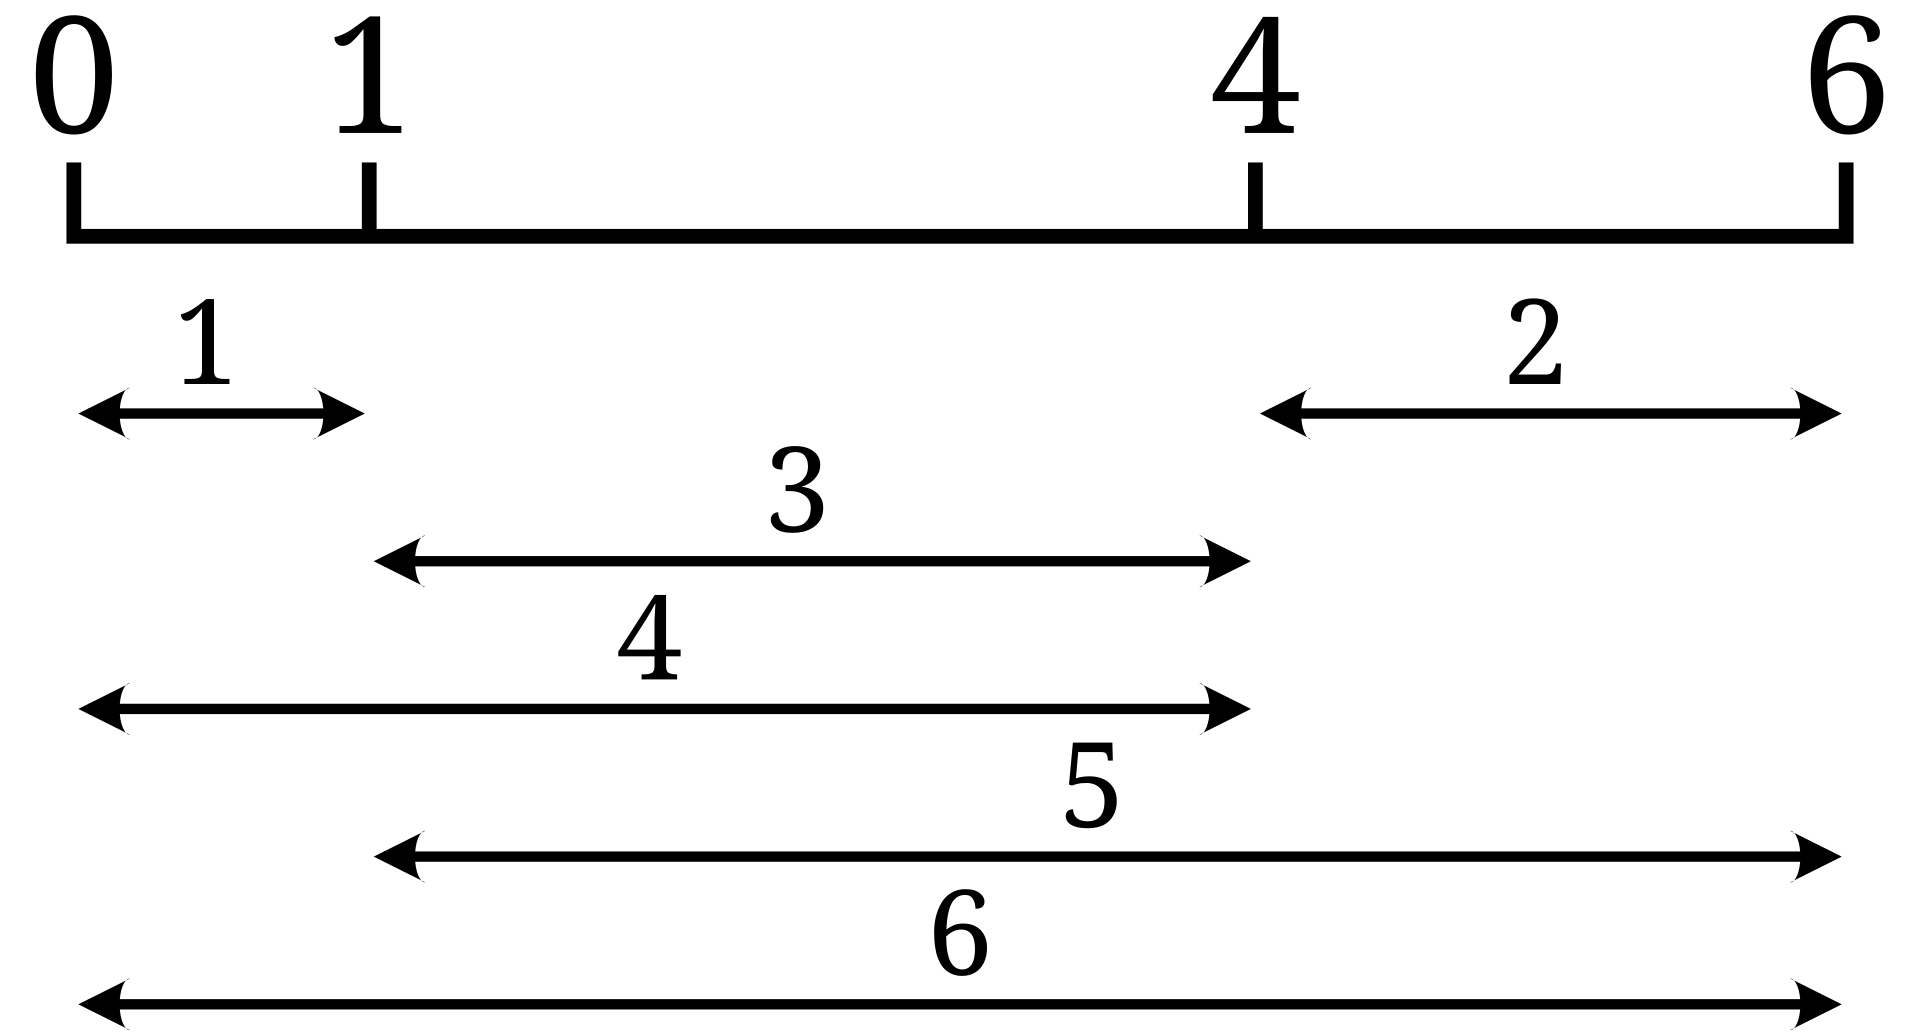
\includegraphics[width=\textwidth]{images/Golomb_Ruler-4.png}%
          \caption{A Golomb ruler for $m=4$ where $x=\sequence{0,1,4,6}$}
        \end{figure}
        \vfill
      \end{center}
    \end{column}
  \end{columns}
\end{example}
\end{frame}

\begin{frame}{What about the Student Seating problem?}
\vfill
\alert{Try it in the exercise session}
\vfill
\end{frame}

\section{Modelling guidelines}

\begin{frame}{From a Problem to a Model}
What is a good model for a constraint problem? \vfill
\begin{itemize}
  \item A model that \alert{correctly} represents the problem \vfill
  \item A model that is \alert{easy} to understand and maintain \vfill
  \item A model that is solved \alert{efficiently}, that is: \vfill
    \begin{itemize}
      \item \alert{short} solving time to find one, all, or best
        solution(s) \vfill
      \item \alert{good} solution within a limited amount of time \vfill
      \item \alert{small} search space (under systematic search)
    \end{itemize}
\end{itemize}\vfill

Food for thought: what is \alert{correct}, \alert{easy},
\alert{short}, \alert{good}, \dots?
\end{frame}

\begin{frame}{Modelling Issues}
Modelling is still more a craft than a science: \vfill
\begin{itemize}
  \item Choice of viewpoint:
    \begin{itemize}
      \item which are the decision variables and their domains? \vfill
      \item will we use different viewpoints for different constraints? \vfill
    \end{itemize}
  \item Choice of the constraint formulations \vfill
  \item Choice of solver and solver configuration (later lectures)
\end{itemize}\vfill

\alert{Make a model correct before making it efficient!}
\end{frame}

\begin{frame}{Tip: declare the Decision Variables with Tight
Domains}\label{tight}
\alert{Tight domains for decision variables might accelerate the
solving.} \vfill
\vspace{1em}

Think about the bounds of your integer variables, avoid lazily
putting a generic large constant.
\begin{example}[Think about tight domains]
  If you have decision variable $x \in \{1, \dots, 20\}$ and $y \in
  \{5, \dots, 10\}$, then if you want to create an explicit
  decision variable with $z = \cons{max}{x,y}$, think it through: \\
  \vspace{-1.5em}
  \begin{align*}
    & z \in \{5, \dots, 20\} \\
    & z = \cons{max}{x,y}    \\
    & \minimize z
  \end{align*}
  \vspace{-1.5em}

  If your modeling library allows it, even better is to use nested expressions; the library will decompose and create an auxiliary variable only if the solver needs it: \\
  \centering
  $\minimize \cons{max}{x,y}$
\end{example}
\end{frame}

\ignore{
\begin{frame}{Tip: beware of non-linear Constraints}
\alert{Constraining the product of two or more decision variables
  often makes
the solving slow.}  Try and find a linear reformulation if
possible.  \vfill

\begin{example}
  For Boolean variables $x, y, z \in \set{0,1}$, the constraint:

  $$x*y + z >= 1$$

  is equivalent to:
  \pause

  $$\Iversion{x \land y} + z >= 1$$
\end{example}
\end{frame}
}

\begin{frame}{Tip: beware of Division Constraints}
\alert{The use of \textit{division} and \textit{modulo} on decision
variables often makes the solving slow.} \\
Reformulate where possible.
\vfill

\begin{example}[Avoid unnecessary divisions]
  If you want to minimize the (integer) average value of an array
  of decision variables $X$:
  \[
    \minimize \sum X / \mathtt{len}(X)
  \]

  then realizing that $\mathtt{len}(X)$ is a constant, you can
  reformulate the objective as:
  \[
    \minimize \sum X
  \]
  given that you post-process the objective value by dividing it by
  $\mathtt{len}(X)$.
\end{example}
\end{frame}

\begin{frame}{Tip: avoid floating point constants in pure integer models}
\begin{example}[]
  The following constraint is inefficient or unsupported for many solvers:
  \[
    \sum X \geq (2/3) \cdot b
  \]

  Instead, bring the denominator to the other side:
  \[
    3\cdot \sum X \geq 2\cdot b
  \]
\end{example}
\end{frame}

\begin{frame}{Summary}
\begin{itemize}
  \item Find the different viewpoints that can be used to model
    the problem
    \begin{itemize}
      \item Is one of them clearly better at formulating the constraints?
      \item Do they give better propagation on a part of the problem?
      \item Should you combine viewpoints?
    \end{itemize}
  \item Express the problem concisely: global constraints and functions
  \item Possibly use redundant constraints to speed up the search
  \item Use few decision variables, and declare tight domains
    \begin{itemize}
      \item Auxiliary variables may be needed to formulate some of the constraints
    \end{itemize}
  \item Beware of division constraints and floating-point values
\end{itemize}
\vfill

Above all: have fun and try different things!
\end{frame}

\end{document}
